\documentclass[conference]{IEEEtran}
\usepackage[utf8]{inputenc}
\usepackage{amsmath,amssymb,graphicx,booktabs}

\usepackage[hidelinks,unicode,pdftitle={Merging Qwen2.5-0.5B-Instruct with Qwen2.5-Coder-0.5B-Instruct: Weighted Sums, TIES and DARE Fall Below Both Parents, and the Coder Task Vector Is 13 Times Larger},pdfauthor={Dheiver Francisco Santos},pdfkeywords={model merging, task arithmetic, TIES, DARE, task vectors, Qwen2.5},pdfsubject={Preprint, Figshare, doi:10.6084/m9.figshare.35013991}]{hyperref}
\begin{document}

\title{Merging Qwen2.5-0.5B-Instruct with Qwen2.5-Coder-0.5B-Instruct: Weighted Sums, TIES and DARE Fall Below Both Parents, and the Coder Task Vector Is 13 Times Larger}

\author{\IEEEauthorblockN{Dheiver Francisco Santos, PhD}
\IEEEauthorblockA{Independent Researcher\\
Maceió, Alagoas, Brazil\\
ORCID: https://orcid.org/0000-0002-8599-9436\\
Preprint, Figshare, 2026, \href{https://doi.org/10.6084/m9.figshare.35013991}{doi:10.6084/m9.figshare.35013991}, CC BY 4.0}}

\maketitle

\begin{abstract}
We test whether a three-model merge of Qwen2.5-0.5B (base), Qwen2.5-0.5B-Instruct and Qwen2.5-Coder-0.5B-Instruct beats the best original model and the best two-model merge. The pre-registered grid (weights from 0.25 up) covers weighted sums, TIES (density 0.5) and DARE ($p=0.5$, five seeds). Selection used 1{,}199 validation items; we report 3{,}967 disjoint test items (macro accuracy over four benchmarks). Hypothesis 4 is rejected twice within the pre-registered grid. The validation-selected weighted sum scores 0.3855, which is $-11.69$ pp [$-13.36$, $-10.00$] against the best original model (base, 0.5025) and $-12.35$ pp [$-14.07$, $-10.67$] against the best two-model merge (LERP, $t=0.7$). TIES and DARE fall further, and every tested merge is below the Coder alone. An exploratory measurement gives the Coder task vector 13 times the relative norm of the Instruct vector. This is consistent with the failure, but no intervention tested the cause. The Coder's initial checkpoint was assumed to be the base (not verified), and the norm ratio and cosine depend on it. One model family at 0.5B scale.
\end{abstract}

\begin{IEEEkeywords}
model merging, task arithmetic, TIES, DARE, task vectors, Qwen2.5
\end{IEEEkeywords}

\section{Introduction}
Merging fine-tuned language models in weight space is attractive because it needs no data and no training. The common recipe adds scaled task vectors, the differences between fine-tuned and base weights, to the base model \cite{ilharco2022editing}. TIES and DARE were designed to reduce interference between such vectors by trimming and sign election \cite{yadav2023ties} or by random dropping with rescaling \cite{yu2023dare}. DARE relies on delta parameters being small and redundant \cite{yu2023dare}, and TIES trims small-magnitude updates and resolves sign conflicts \cite{yadav2023ties}. Small deltas are natural for a short fine-tune, but not guaranteed for public checkpoints that practitioners merge in practice.

Qwen2.5-Coder-0.5B-Instruct \cite{hui2024qwen25coder} is such a case. Its technical report describes a code-specialized model obtained by continued training of Qwen2.5 \cite{yang2024qwen25} rather than a brief fine-tune. It shares architecture and tokenizer with Qwen2.5-0.5B and Qwen2.5-0.5B-Instruct, so the three can be merged tensor by tensor, and the toolkits that implement the standard recipes \cite{goddard2024mergekit} would accept them without complaint.

The pre-registered hypothesis (H4) is that a three-model merge beats the best two-model merge; we also test the general-rule baseline, the best original model. So we ask: can a weighted three-model merge, TIES, or DARE beat either, on benchmark items never used for selection? We find that it cannot, by a wide margin. We also report an exploratory measurement of the task vectors that is consistent with one explanation. That explanation remains a conjecture, because we ran no intervention that isolates it.

\section{Related Work}
\textbf{Task vectors and arithmetic.} Task arithmetic edits a model by adding or subtracting scaled differences between fine-tuned and pre-trained weights \cite{ilharco2022editing}. Ortiz-Jimenez et al.\ argue that its success depends on weight disentanglement, which holds more clearly in a tangent-space (linearized) regime \cite{ortizjimenez2023tangent}. Chat Vector transfers instruction-following by adding the difference between a chat model and its base \cite{huang2023chatvector}, again for a vector obtained by fine-tuning from that base. Earlier weight-averaging and fusion work \cite{wortsman2022soups,jin2022dataless,matena2021fisher} merges fine-tunes of one initialization; we read this as a closeness-in-weight-space condition (our interpretation), related to linear mode connectivity \cite{frankle2019lmc}.

\textbf{Interference between task vectors.} TIES-Merging identifies two sources of interference: redundant small-magnitude parameters and sign conflicts, and resolves them by trimming, sign election and a disjoint mean \cite{yadav2023ties}. DARE drops a random fraction $p$ of delta parameters and rescales the rest by $1/(1-p)$, and relies on delta parameters being small and redundant \cite{yu2023dare}. A study of merging at scale examines how base-model quality and model size affect merging outcomes \cite{yadav2024matters}, a survey covers task arithmetic, TIES and DARE \cite{yang2024survey}, and another surveys deep model fusion more broadly \cite{li2023fusion}. These works motivate our test but do not test merges where one vector is more than ten times larger than the other.

\textbf{Toolkits and automated search.} MergeKit packages linear, SLERP, TIES and DARE-style merges for public checkpoints \cite{goddard2024mergekit}. Evolutionary model merging searches merge recipes automatically, in both parameter space and data-flow space, and reports successful merges of models from different domains \cite{akiba2024evolutionary}. Those results show that merging across domains can work after search, but they do not say when a fixed, pre-specified recipe will fail.

\textbf{Qwen2.5-Coder.} The Qwen2.5-Coder report documents code-specific continued training and instruction tuning, reportedly built on the Qwen2.5 base \cite{hui2024qwen25coder}. The gap we occupy is a controlled, held-out measurement of the standard fixed recipes on exactly this pair, reported with the task-vector geometry measured on the same checkpoints.

\textbf{Author's related work.} The author's technical notes cover neighboring topics in language-model training: model merging for capability composition \cite{santos2026modelmergingfo}, mixture-of-experts training and sparse upcycling \cite{santos2026mixtureofexper}, knowledge distillation and self-distillation \cite{santos2026knowledgedisti}, parameter-efficient fine-tuning (LoRA, QLoRA, DoRA) \cite{santos2026parametereffic}, curriculum learning and data-efficient pretraining \cite{santos2026curriculumlear}, synthetic data generation and self-improvement \cite{santos2026syntheticdatag}, direct preference optimization \cite{santos2026directpreferen}, and RLAIF and Constitutional AI \cite{santos2026rlaifandconsti}. This paper instead reports a controlled held-out measurement. In a different domain, the author's JEPA preprint \cite{santos2026collapseresist} uses a similar controlled-comparison style (identical budgets, several seeds, confidence intervals).

\section{Method}
Let $\theta_0$ be the base weights (Qwen2.5-0.5B), and $\theta_I$, $\theta_C$ the weights of the Instruct and Coder-Instruct models. Define task vectors $\tau_I=\theta_I-\theta_0$ and $\tau_C=\theta_C-\theta_0$. The Coder vector is taken relative to the Qwen2.5-0.5B base, the checkpoint the Coder family is built on; we did not verify the Coder's exact initial checkpoint. All merges below have the form $\theta_0+\sum_k\lambda_k\tau_k$ with different treatment of $\tau_k$.

\textbf{Weighted sum.} $\theta=\theta_0+\lambda_I\tau_I+\lambda_C\tau_C$ with $\lambda_I,\lambda_C\in\{0.25,0.5,0.75\}$ (nine configurations).

\textbf{TIES.} Each $\tau_k$ is trimmed to its top 50\% entries by magnitude (per tensor), the sign of each entry is elected by the sign of the summed trimmed vectors, and entries that agree with the elected sign are averaged (disjoint mean); the merged vector is added with $\lambda=1$.

\textbf{DARE.} $\tilde\tau_k=(m_k\odot\tau_k)/(1-p)$ with $m_k$ i.i.d.\ Bernoulli$(1-p)$ masks, $p=0.5$, independent per vector, and the merge is $\theta_0+0.5\tilde\tau_I+0.5\tilde\tau_C$. Seeds $s=0,\dots,4$ change the masks.

\subsection*{Equations and their meaning}
\begin{equation}
\theta_{\text{merge}}=\theta_0+\lambda_I\,\tau_I+\lambda_C\,\tau_C,\qquad \tau_k=\theta_k-\theta_0 .
\end{equation}
The merged model starts at the base and moves a fraction $\lambda_k$ along each fine-tuning direction. With $\lambda_I=\lambda_C=0.5$ this is exactly the average of the two fine-tuned models.
\begin{equation}
\rho_k=\frac{\lVert\tau_k\rVert_2}{\lVert\theta_0\rVert_2},\qquad
\cos(\tau_I,\tau_C)=\frac{\langle\tau_I,\tau_C\rangle}{\lVert\tau_I\rVert_2\lVert\tau_C\rVert_2}.
\end{equation}
The relative norm $\rho_k$ tells how far a fine-tuned model sits from the base in units of the base weights' own size; the cosine tells whether the two moves point in different directions. Both are computed over all parameters flattened into one vector, with double-precision accumulation.
\begin{equation}
\mathbb{E}\,\big\lVert\tilde\tau-\tau\big\rVert_2^2=\frac{p}{1-p}\,\lVert\tau\rVert_2^2 .
\end{equation}
This identity for the DARE rescaled mask (a one-line consequence of the Bernoulli variance) says that the expected squared error injected into the weights is proportional to $\lVert\tau\rVert_2^2$. At $p=0.5$ the factor is 1, so the error has the same expected norm as $\tau$ itself, 100\% of $\lVert\tau\rVert_2$ for any vector. What differs between vectors is only the absolute scale relative to $\lVert\theta_0\rVert_2$. As a heuristic, a larger absolute error is more likely to matter; we never tested a threshold.
\begin{equation}
\Delta=\overline{a}_{\text{merge}}-\overline{a}_{\text{base}},\quad \overline{a}=\tfrac14\sum_{j=1}^{4}\text{acc}_j .
\end{equation}
The reported effect is the difference of macro accuracies (mean over the four tasks, tasks weighted equally), paired by test item.

\section{Experimental Protocol}
\textbf{Models.} Qwen2.5-0.5B (base, Hub commit 060db64), Qwen2.5-0.5B-Instruct (7ae5576) and Qwen2.5-Coder-0.5B-Instruct (ea3f247), all Apache-2.0 \cite{yang2024qwen25,hui2024qwen25coder}. Merging is done in fp32 on CPU and copied into a bf16 model for evaluation.

\textbf{Data and splits.} Multiple-choice benchmarks scored by log-likelihood in the style of the lm-evaluation-harness \cite{gao2021harness}: ARC-Easy and ARC-Challenge \cite{clark2018arc}, HellaSwag \cite{zellers2019hellaswag} and WinoGrande \cite{sakaguchi2019winogrande}. Validation has 300 items per task (299 for ARC-Challenge, 1{,}199 in total); test has 1{,}000 per task (967 for WinoGrande, 3{,}967 in total). Splits are disjoint and fixed with seed 0. The metric is the macro mean of the four accuracies.

\textbf{Selection.} Pre-registered before any merge was run (hypothesis 4): grid $\lambda_I,\lambda_C\in\{0.25,0.5,0.75\}^2$, TIES with density 0.5, $\lambda=1$, and DARE with $p=0.5$ and five seeds. The best grid point was chosen on validation and was the only grid point whose test items were read, together with the Coder, the TIES merge, the average, and the five DARE seeds. No grid, metric or hypothesis was changed after seeing results.

\textbf{Baselines.} The best original model chosen on validation, which is the base model (validation 0.4953 against 0.4853 for Instruct). The Coder alone and the average were not in the pre-registration: they are baselines added for reference. The best pre-registered two-model merge (base--Instruct interpolation with $t=0.7$) is the baseline of hypothesis 4.

\textbf{Statistics.} Item-level bootstrap \cite{efron1979bootstrap,miller2024errorbars} (2000 resamples for a single accuracy, 3000 for paired differences), tasks weighted equally, bootstrap two-sided $p$. A $p$ reported as $<0.001$ means no resample crossed zero (B$=$3{,}000: the smallest nonzero two-sided $p$ is $2/3{,}000$). The pre-registration (\texttt{experiments/PREREG.md}) fixed 5{,}000 bootstrap resamples; the analysis used 2{,}000 for a single accuracy and 3{,}000 for paired differences (5{,}000 for per-block NLL differences, Articles 7 and 10). The primary comparison for this article is the selected merge against the best original; the Bonferroni threshold for the six primary comparisons across Articles 1--6 is $0.05/6=0.0083$. It was added after the pre-registration, whose success rule was a paired 95\% CI above zero. DARE variability is the sample standard deviation (ddof$=$1) over five mask seeds.

\section{Results}
Table~\ref{tab:all} lists every configuration. Test results exist only for configurations selected on validation (the best weighted sum) or specified in advance (TIES, DARE), or added as reference baselines (Coder, average); the other grid points have validation scores only, by design.

\begin{table*}[!t]
\caption{All configurations. Validation (1{,}199 items) macro accuracy; test (3{,}967 items) macro accuracy with 95\% bootstrap CI; paired difference to the base model in percentage points with 95\% CI and bootstrap $p$. Dashes: test items were not read for that configuration (protocol). The Avg row equals the grid point $\lambda_I=\lambda_C=0.5$.}
\label{tab:all}
\centering\small
\begin{tabular}{lcccc}
\toprule
Configuration & Val. & Test [95\% CI] & $\Delta$ vs.\ base (pp) [95\% CI] & $p$ \\
\midrule
Qwen2.5-0.5B (base) & 0.4953 & 0.5025 [0.4875, 0.5174] & reference &  \\
Qwen2.5-0.5B-Instruct & 0.4853 & 0.5064 [0.4909, 0.5220] & +0.40 [$-$0.62, +1.41] & 0.441 \\
Coder-0.5B-Instruct & 0.3977 & 0.4042 [0.3892, 0.4199] & $-$9.82 [$-$11.34, $-$8.17] & $<$0.001 \\
LERP(base,instruct), t=0.7 & 0.4961 & 0.5090 [0.4938, 0.5246] & +0.65 [$-$0.23, +1.52] & 0.149 \\
\midrule
3-way $\lambda_I$=0.25, $\lambda_C$=0.25 & 0.3527 & -- & -- & -- \\
3-way $\lambda_I$=0.25, $\lambda_C$=0.5 & 0.3402 & -- & -- & -- \\
3-way $\lambda_I$=0.25, $\lambda_C$=0.75 & 0.3677 & -- & -- & -- \\
3-way $\lambda_I$=0.5, $\lambda_C$=0.25 & 0.3577 & -- & -- & -- \\
3-way $\lambda_I$=0.5, $\lambda_C$=0.5 & 0.3394 & -- & -- & -- \\
3-way $\lambda_I$=0.5, $\lambda_C$=0.75 & 0.3685 & -- & -- & -- \\
3-way $\lambda_I$=0.75, $\lambda_C$=0.25 & 0.3519 & -- & -- & -- \\
3-way $\lambda_I$=0.75, $\lambda_C$=0.5 & 0.3402 & -- & -- & -- \\
3-way $\lambda_I$=0.75, $\lambda_C$=0.75 & 0.3852 & 0.3855 [0.3711, 0.4009] & $-$11.69 [$-$13.36, $-$10.00] & $<$0.001 \\
\midrule
Avg(instruct, coder) & 0.3394 & 0.3418 [0.3278, 0.3575] & $-$16.06 [$-$17.91, $-$14.19] & $<$0.001 \\
TIES (d=0.5) & 0.3294 & 0.3322 [0.3180, 0.3470] & $-$17.02 [$-$18.90, $-$15.13] & $<$0.001 \\
\midrule
DARE (p=0.5), seed 0 & 0.2985 & 0.3183 [0.3047, 0.3317] & $-$18.41 [$-$20.41, $-$16.44] & $<$0.001 \\
DARE (p=0.5), seed 1 & 0.2985 & 0.3246 [0.3101, 0.3398] & $-$17.78 [$-$19.71, $-$15.78] & $<$0.001 \\
DARE (p=0.5), seed 2 & 0.3069 & 0.3214 [0.3068, 0.3362] & $-$18.11 [$-$20.11, $-$16.11] & $<$0.001 \\
DARE (p=0.5), seed 3 & 0.3177 & 0.3169 [0.3028, 0.3313] & $-$18.55 [$-$20.54, $-$16.56] & $<$0.001 \\
DARE (p=0.5), seed 4 & 0.2869 & 0.3198 [0.3053, 0.3344] & $-$18.27 [$-$20.32, $-$16.30] & $<$0.001 \\
\bottomrule
\end{tabular}
\end{table*}

\textbf{Hypothesis 4 is rejected, against both baselines.} The pre-registered hypothesis was that the three-model merge beats the best two-model merge; it also fails against the best original model. The selected weighted sum ($\lambda_I=\lambda_C=0.75$) scores 0.3855 on test, $-11.69$ pp [$-13.36$, $-10.00$] against the base (bootstrap $p<0.001$, well below 0.0083), and $-12.35$ pp [$-14.07$, $-10.67$] against the best pre-registered two-model merge. It is also below the Coder alone by $-1.87$ pp [$-3.25$, $-0.51$] ($p=0.005$ nominal). Simple averaging ($\lambda_I=\lambda_C=0.5$, which coincides with the grid point of the same name, validation 0.3394 in both rows) reaches 0.3418. TIES reaches 0.3322. DARE over five seeds gives $0.3202\pm0.0030$ on test (range 0.3169 to 0.3246) and $0.3017\pm0.0114$ on validation. Every DARE seed is 17.8 to 18.6 pp below the base with intervals excluding zero. Several merged models are at or near chance on individual tasks: for example TIES reaches 0.296 on ARC-Easy and 0.231 on ARC-Challenge (four options, chance 0.25).

\begin{figure}[!t]
\centering
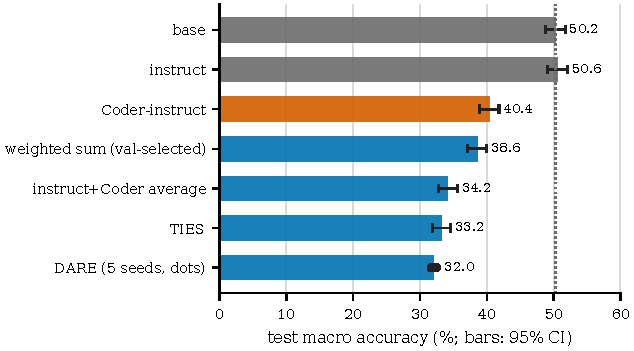
\includegraphics[width=\columnwidth]{figs/fig04_threeway.pdf}
\caption{Test macro accuracy with 95\% CI on 3{,}967 items: originals grey, Coder orange, merges blue. DARE shows its five seeds as points and their mean as the bar. Dotted line: base. Every merge lies below the base and the Instruct model.}
\label{fig:fig04_threeway}
\end{figure}

\textbf{Measured task-vector geometry (exploratory).} The relative norm of the Instruct vector is $\rho_I=0.0418$; that of the Coder vector is $\rho_C=0.5614$, a factor of 13.4. The cosine between them is 0.140. For a 0.5B-parameter model, a cosine of 0.140 is far from what random directions would give ($\approx 5\times10^{-5}$), so the vectors are not orthogonal in the strict sense, only weakly aligned. For reference, the SmolLM2-360M Instruct vector has $\rho=0.0794$ (single measurement on another family). By Eq.~(3), DARE at $p=0.5$ with weight 0.5 adds expected random error of relative size $0.5\sqrt{\rho_I^2+\rho_C^2}\approx0.28$ to the weights, against $0.021$ for the Instruct vector alone. These are absolute scales only; the error is 100\% of $\lVert\tau\rVert$ in both cases, and we never applied DARE to the Instruct vector alone, so we do not know that $0.021$ is harmless.

\textbf{What this does and does not show.} One reading is that the merges fail because the Coder vector is not small: it reflects a long continuation of training, so the premises of the methods (small, redundant, roughly non-interfering deltas) may not hold. The measured norm and cosine are consistent with this. The Coder alone already loses 9.82 pp [$-11.34$, $-8.17$] against the base on these benchmarks, so part of the loss may simply be the Coder's own. The causal claim is not demonstrated: no intervention tested it. We did not use $\lambda_C<0.25$, apply DARE to the Instruct vector alone, shrink the Coder vector, or run a short code fine-tune. The result also does not say that the Coder is a poor model; these benchmarks measure commonsense and science knowledge, not code.

\section{Discussion and Limitations}
\textbf{Grid design.} The pre-registered grid has a lower bound of 0.25. Merges close to the base (for instance $\lambda_C<0.25$) were not tested and would be expected to approach the base or the two-model merge; our claim is about the pre-registered recipes only. The best grid point lies at the grid corner. Its $\lambda_I+\lambda_C=1.5>1$, so it mixes merging with extrapolation of both vectors; Article 3 detects no improvement at $\lambda=1.5$ for the Instruct vector alone. Validation is non-monotonic in $\lambda_C$ ($0.3527$, $0.3402$, $0.3677$ at $\lambda_I=0.25$), which we do not explain.

\textbf{Scope.} One model family, 0.5B parameters, four benchmarks of commonsense and science multiple choice, one hardware (Apple Silicon, bf16), one split seed. The test set is slightly easier than validation (about 0.50 against 0.495 for the base), so comparisons use gains, not levels. Possible benchmark contamination in the pretrained models is not controlled. TIES was run at a single density and DARE at a single $p$; other settings may behave differently. The Coder's initial checkpoint was assumed, not verified. All evaluations used bfloat16. Re-evaluating validation accuracy in fp32 at $t=0$, $0.7$ and $1$ (where $t$ is the base--Instruct interpolation coefficient, $\theta_0+t\tau_I$) lowered the macro accuracy by $0.67$, $0.41$ and $0.08$~pp (fp32: $0.4886$, $0.4920$, $0.4845$), a shift of the same size as the differences between coefficients, while the order of the three points did not change and WikiText-2 NLL moved by at most $0.0026$ nats at any $t$ (\texttt{results/fp32\_check\_qwen.txt}). Exact accuracy levels are therefore specific to bfloat16, and the test items were not re-evaluated in fp32. The check covers only the base--Instruct interpolation ($t=0$, $0.7$, $1$), not the three-model merges or the Coder. The effects of this paper (11--18 pp) are insensitive to a shift of $0.7$ pp. The 0.5614 norm is one number from one pair; the explanation of Section V is a conjecture supported by it, not a test of it. Multiple-testing: the nominal $p$ values in Table~\ref{tab:all} other than the primary comparison are descriptive.

\section{Conclusion}
On Qwen2.5-0.5B, the pre-registered weighted sum, TIES and DARE merges of the base, Instruct and Coder-Instruct models all fall 11.7 to 18.6 pp below the best original model on 3{,}967 held-out items. They also fall below the Coder alone. The Coder task vector is 13 times larger than the Instruct vector (relative norm 0.5614 against 0.0418), with cosine 0.140. This is consistent with a violation of the small-vector premise of the methods, but no intervention tested the cause; the Coder alone already loses 9.82 pp against the base. Practitioners should measure task-vector norms before merging and should not assume that a public domain-specialized checkpoint behaves like a short fine-tune.

\section*{Data and Code Availability}
Code, per-item caches and tables are in the repository at git tag \texttt{preprints-v1} (the commit that contains this manuscript and all scripts and caches); new scripts for the tables here are \texttt{experiments/an\_art04\_05\_tables.py} (output \texttt{results/tables\_art04\_05.json}), with \texttt{experiments/an\_taskvec.py} for the geometry (\texttt{results/taskvec.json}). A single command regenerates all results and tables: \texttt{./run\_everything.sh}. Software: Python 3.9.6, PyTorch 2.8.0, transformers 4.57.6, NumPy 1.26.4, datasets 4.5.0. Model revisions (Hub commits, full hashes in \texttt{MANIFEST.json}): Qwen2.5-0.5B 060db6499f32, Qwen2.5-0.5B-Instruct 7ae557604adf, Qwen2.5-Coder-0.5B-Instruct ea3f2471cf1b. Seeds: split seed 0; DARE seeds 0 to 4; bootstrap seed 0.

\section*{Acknowledgments}
No external funding.

\begin{thebibliography}{99}
\bibitem{ilharco2022editing} G. Ilharco, M. T. Ribeiro, M. Wortsman et al., ``Editing models with task arithmetic,'' in \emph{Proc.\ ICLR}, 2023, arXiv:2212.04089.
\bibitem{yadav2023ties} P. Yadav, D. Tam, L. Choshen et al., ``TIES-Merging: Resolving interference when merging models,'' in \emph{Proc.\ NeurIPS}, 2023, arXiv:2306.01708.
\bibitem{yu2023dare} L. Yu, B. Yu, H. Yu et al., ``Language models are Super Mario: Absorbing abilities from homologous models as a free lunch,'' in \emph{Proc.\ ICML}, 2024, arXiv:2311.03099.
\bibitem{ortizjimenez2023tangent} G. Ortiz-Jimenez, A. Favero, and P. Frossard, ``Task arithmetic in the tangent space: Improved editing of pre-trained models,'' in \emph{Proc.\ NeurIPS}, 2023, arXiv:2305.12827.
\bibitem{huang2023chatvector} S.-C. Huang, P.-Z. Li, Y.-C. Hsu et al., ``Chat Vector: A simple approach to equip LLMs with instruction following and model alignment in new languages,'' in \emph{Proc.\ ACL}, 2024, arXiv:2310.04799.
\bibitem{wortsman2022soups} M. Wortsman, G. Ilharco, S. Y. Gadre et al., ``Model soups: Averaging weights of multiple fine-tuned models improves accuracy without increasing inference time,'' in \emph{Proc.\ ICML}, 2022, arXiv:2203.05482.
\bibitem{jin2022dataless} X. Jin, X. Ren, D. Preotiuc-Pietro et al., ``Dataless knowledge fusion by merging weights of language models,'' in \emph{Proc.\ ICLR}, 2023, arXiv:2212.09849.
\bibitem{matena2021fisher} M. Matena and C. Raffel, ``Merging models with Fisher-weighted averaging,'' arXiv:2111.09832, 2021.
\bibitem{yadav2024matters} P. Yadav, T. Vu, J. Lai et al., ``What matters for model merging at scale?'' arXiv:2410.03617, 2024.
\bibitem{yang2024survey} E. Yang, L. Shen, G. Guo et al., ``Model merging in LLMs, MLLMs, and beyond: Methods, theories, applications and opportunities,'' arXiv:2408.07666, 2024.
\bibitem{goddard2024mergekit} C. Goddard, S. Siriwardhana, M. Ehghaghi et al., ``Arcee's MergeKit: A toolkit for merging large language models,'' arXiv:2403.13257, 2024.
\bibitem{akiba2024evolutionary} T. Akiba, M. Shing, Y. Tang et al., ``Evolutionary optimization of model merging recipes,'' \emph{Nat.\ Mach.\ Intell.}, 2025, arXiv:2403.13187.
\bibitem{hui2024qwen25coder} B. Hui, J. Yang, Z. Cui et al., ``Qwen2.5-Coder technical report,'' arXiv:2409.12186, 2024.
\bibitem{yang2024qwen25} Qwen Team, A. Yang et al., ``Qwen2.5 technical report,'' arXiv:2412.15115, 2024.
\bibitem{frankle2019lmc} J. Frankle, G. K. Dziugaite, D. M. Roy et al., ``Linear mode connectivity and the lottery ticket hypothesis,'' in \emph{Proc.\ ICML}, 2020, arXiv:1912.05671.
\bibitem{li2023fusion} W. Li, Y. Peng, M. Zhang et al., ``Deep model fusion: A survey,'' arXiv:2309.15698, 2023.
\bibitem{clark2018arc} P. Clark, I. Cowhey, O. Etzioni et al., ``Think you have solved question answering? Try ARC, the AI2 Reasoning Challenge,'' arXiv:1803.05457, 2018.
\bibitem{zellers2019hellaswag} R. Zellers, A. Holtzman, Y. Bisk et al., ``HellaSwag: Can a machine really finish your sentence?'' in \emph{Proc.\ ACL}, 2019, arXiv:1905.07830.
\bibitem{sakaguchi2019winogrande} K. Sakaguchi, R. Le Bras, C. Bhagavatula et al., ``WinoGrande: An adversarial Winograd schema challenge at scale,'' arXiv:1907.10641, 2019.
\bibitem{gao2021harness} L. Gao et al., ``EleutherAI/lm-evaluation-harness,'' Zenodo, doi:10.5281/zenodo.10256836.
\bibitem{miller2024errorbars} E. Miller, ``Adding error bars to evals: A statistical approach to language model evaluations,'' arXiv:2411.00640, 2024.
\bibitem{efron1979bootstrap} B. Efron, ``Bootstrap methods: Another look at the jackknife,'' \emph{Ann. Statist.}, 1979, doi:10.1214/aos/1176344552.
\bibitem{santos2026modelmergingfo} D. F. Santos, ``Model Merging for Capability Composition: A Technical Note,'' Zenodo, 2026, doi:10.5281/zenodo.21610555.
\bibitem{santos2026collapseresist} D. F. Santos, ``Collapse-Resistant Joint-Embedding Predictive Architectures: A Controlled Comparison of SIGReg, VICReg, and EMA,'' Zenodo, v2, 2026, doi:10.5281/zenodo.24223364.
\bibitem{santos2026mixtureofexper} D. F. Santos, ``Mixture-of-Experts Training and Sparse Upcycling,'' Zenodo, 2026, doi:10.5281/zenodo.21610062.
\bibitem{santos2026knowledgedisti} D. F. Santos, ``Knowledge Distillation and Self-Distillation for Language Models,'' Zenodo, 2026, doi:10.5281/zenodo.21610100.
\bibitem{santos2026parametereffic} D. F. Santos, ``Parameter-Efficient Fine-Tuning: LoRA, QLoRA, and DoRA,'' Zenodo, 2026, doi:10.5281/zenodo.21610033.
\bibitem{santos2026curriculumlear} D. F. Santos, ``Curriculum Learning and Data-Efficient Pretraining: A Technical Note,'' Zenodo, 2026, doi:10.5281/zenodo.21610595.
\bibitem{santos2026syntheticdatag} D. F. Santos, ``Synthetic Data Generation and Self-Improvement: A Technical Note,'' Zenodo, 2026, doi:10.5281/zenodo.21610525.
\bibitem{santos2026directpreferen} D. F. Santos, ``Direct Preference Optimization (DPO): A Technical Note,'' Zenodo, 2026, doi:10.5281/zenodo.21609911.
\bibitem{santos2026rlaifandconsti} D. F. Santos, ``RLAIF and Constitutional AI: A Technical Note,'' Zenodo, 2026, doi:10.5281/zenodo.21610280.
\end{thebibliography}

\end{document}
